% Options for packages loaded elsewhere
\PassOptionsToPackage{unicode}{hyperref}
\PassOptionsToPackage{hyphens}{url}
\PassOptionsToPackage{dvipsnames,svgnames*,x11names*,table}{xcolor}
%
\documentclass[
  13pt,
  %% For koma-script
  fontsize=13pt,
  russian,
  a4paper,
,captions=tableheading
]{scrreprt}
\usepackage{amsmath,amssymb}
\usepackage{lmodern}
\usepackage{setspace}
\usepackage{ifxetex,ifluatex}
\ifnum 0\ifxetex 1\fi\ifluatex 1\fi=0 % if pdftex
  \usepackage[T1]{fontenc}
  \usepackage[utf8]{inputenc}
  \usepackage{textcomp} % provide euro and other symbols
\else % if luatex or xetex
  \usepackage{unicode-math}
  \defaultfontfeatures{Scale=MatchLowercase}
  \defaultfontfeatures[\rmfamily]{Ligatures=TeX,Scale=1}
  \setmainfont[Ligatures=TeX]{PT Serif}
  \setsansfont[Ligatures=TeX,Scale=MatchLowercase]{PT Sans}
  \setmonofont[Scale=MatchLowercase,Scale=0.9]{PT Mono}
\fi
% koma-script tuning
\KOMAoptions{twoside=false}
\KOMAoptions{headings=standardclasses}
\KOMAoptions{headings=small}
\KOMAoptions{chapterprefix=false}
\renewcommand*{\chapterheadstartvskip}{}
% \renewcommand*{\chapterheadendvskip}{\vspace*{2\baselineskip}}
% \renewcommand{\chapterheadstartvskip}{\vspace*{10\baselineskip}}%
\RedeclareSectionCommand[beforeskip=0pt]{chapter}
% \RedeclareSectionCommand[%
% runin=false,
% afterindent=false,
% beforeskip=0pt,
% afterskip=0pt,
% afterskip=2\baselineskip,
% innerskip=0pt,
% ]{chapter}
% \RedeclareSectionCommand[%
% % runin=false,
% afterindent=false,
% beforeskip=\baselineskip,
% afterskip=.5\baselineskip]{section}
% \RedeclareSectionCommand[%
% % runin=false,
% afterindent=false,
% beforeskip=.75\baselineskip,
% afterskip=.5\baselineskip]{subsection}
% \RedeclareSectionCommand[%
% % runin=false,
% afterindent=false,
% beforeskip=.5\baselineskip,
% afterskip=.25\baselineskip]{subsubsection}
% \RedeclareSectionCommand[%
% runin=true,
% % afterindent=false,
% beforeskip=.5\baselineskip,
% afterskip=1em]{paragraph}
% \RedeclareSectionCommand[%
% runin=true,
% % afterindent=false,
% beforeskip=.5\baselineskip,
% afterskip=1em]{subparagraph}
% \setcaptionalignment[figure]{C}
% \setcaptionalignment[table]{R}
% \renewcommand*{\figureformat}{\figurename~\thefigure\autodot}
% \renewcommand*{\tableformat}{\tablename~\thetable\autodot}
\usepackage{enumitem}
\setlist{nosep}
\renewcommand{\labelitemi}{\bfseries\textemdash}                                                                                                                                                                                               
\renewcommand{\labelitemii}{\bfseries\textemdash}                                                                                                                                                                                              
\renewcommand{\labelitemiii}{\bfseries\textemdash}                                                                                                                                                                                             
\renewcommand{\labelitemiv}{\bfseries\textemdash}
%%
% Use upquote if available, for straight quotes in verbatim environments
\IfFileExists{upquote.sty}{\usepackage{upquote}}{}
\IfFileExists{microtype.sty}{% use microtype if available
  \usepackage[]{microtype}
  \UseMicrotypeSet[protrusion]{basicmath} % disable protrusion for tt fonts
}{}
\usepackage{indentfirst}
\usepackage{xcolor}
\definecolor{default-linkcolor}{HTML}{A50000}
\definecolor{default-filecolor}{HTML}{A50000}
\definecolor{default-citecolor}{HTML}{4077C0}
\definecolor{default-urlcolor}{HTML}{4077C0}
\IfFileExists{xurl.sty}{\usepackage{xurl}}{} % add URL line breaks if available
\IfFileExists{bookmark.sty}{\usepackage{bookmark}}{\usepackage{hyperref}}
\hypersetup{
  pdftitle={Модель ``Хищник-жертва'' на загрязненной территории},
  pdfauthor={В. М. Шутенко},
  pdflang={ru-RU},
  hidelinks,
  breaklinks=true,
  pdfcreator={LaTeX via pandoc with the Eisvogel template}}
\urlstyle{same} % disable monospaced font for URLs
\usepackage[left=30mm,right=10mm,top=20mm,bottom=20mm,nohead,includefoot=true]{geometry}

% % \AfterCalculatingTypearea{
%   \newgeometry{%
%   left=30mm,
%   right=15mm,
%   top=20mm,
%   bottom=20mm,
%   % bindingoffset=10mm,
%   % includefoot,
%   % foot=\baselineskip,
%   % showframe
% }
% % }
% % \recalctypearea


\usepackage{longtable,booktabs,array}
\usepackage{calc} % for calculating minipage widths
% Correct order of tables after \paragraph or \subparagraph
\usepackage{etoolbox}
\makeatletter
\patchcmd\longtable{\par}{\if@noskipsec\mbox{}\fi\par}{}{}
\makeatother
% Allow footnotes in longtable head/foot
\IfFileExists{footnotehyper.sty}{\usepackage{footnotehyper}}{\usepackage{footnote}}
\makesavenoteenv{longtable}
% add backlinks to footnote references, cf. https://tex.stackexchange.com/questions/302266/make-footnote-clickable-both-ways
\usepackage{footnotebackref}
\usepackage{graphicx}
\makeatletter
\def\maxwidth{\ifdim\Gin@nat@width>\linewidth\linewidth\else\Gin@nat@width\fi}
\def\maxheight{\ifdim\Gin@nat@height>\textheight\textheight\else\Gin@nat@height\fi}
\makeatother
% Scale images if necessary, so that they will not overflow the page
% margins by default, and it is still possible to overwrite the defaults
% using explicit options in \includegraphics[width, height, ...]{}
\setkeys{Gin}{width=\maxwidth,height=\maxheight,keepaspectratio}
% Set default figure placement to htbp
\makeatletter
\def\fps@figure{htbp}
\makeatother
\setlength{\emergencystretch}{3em} % prevent overfull lines
\providecommand{\tightlist}{%
  \setlength{\itemsep}{0pt}\setlength{\parskip}{0pt}}
\setcounter{secnumdepth}{5}

% Make use of float-package and set default placement for figures to H.
% The option H means 'PUT IT HERE' (as  opposed to the standard h option which means 'You may put it here if you like').
\usepackage{float}
\floatplacement{figure}{H}

\linepenalty=10
\interlinepenalty=0
\hyphenpenalty=50
\exhyphenpenalty=50
\binoppenalty=700
\relpenalty=500
\clubpenalty=150
\widowpenalty=150
\displaywidowpenalty=50
\brokenpenalty=100
\predisplaypenalty=10000
\postdisplaypenalty=0
\floatingpenalty = 20000
\flushbottom
\usepackage{float}
\floatplacement{figure}{bt}
\usepackage{menukeys}
\usepackage{minted}
\usepackage{amsmath}
\usepackage{mathtools}
\usepackage{physics}
\setminted{breaklines}
\graphicspath{{/}{image/}}
\makeatletter
\let\listoflistings\@undefined
\makeatother
\makeatletter
\@ifpackageloaded{subfig}{}{\usepackage{subfig}}
\@ifpackageloaded{caption}{}{\usepackage{caption}}
\captionsetup[subfloat]{margin=0.5em}
\AtBeginDocument{%
\renewcommand*\figurename{Figure}
\renewcommand*\tablename{Table}
}
\AtBeginDocument{%
\renewcommand*\listfigurename{List of Figures}
\renewcommand*\listtablename{List of Tables}
}
\newcounter{pandoccrossref@subfigures@footnote@counter}
\newenvironment{pandoccrossrefsubfigures}{%
\setcounter{pandoccrossref@subfigures@footnote@counter}{0}
\begin{figure}\centering%
\gdef\global@pandoccrossref@subfigures@footnotes{}%
\DeclareRobustCommand{\footnote}[1]{\footnotemark%
\stepcounter{pandoccrossref@subfigures@footnote@counter}%
\ifx\global@pandoccrossref@subfigures@footnotes\empty%
\gdef\global@pandoccrossref@subfigures@footnotes{{##1}}%
\else%
\g@addto@macro\global@pandoccrossref@subfigures@footnotes{, {##1}}%
\fi}}%
{\end{figure}%
\addtocounter{footnote}{-\value{pandoccrossref@subfigures@footnote@counter}}
\@for\f:=\global@pandoccrossref@subfigures@footnotes\do{\stepcounter{footnote}\footnotetext{\f}}%
\gdef\global@pandoccrossref@subfigures@footnotes{}}
\@ifpackageloaded{float}{}{\usepackage{float}}
\floatstyle{ruled}
\@ifundefined{c@chapter}{\newfloat{codelisting}{h}{lop}}{\newfloat{codelisting}{h}{lop}[chapter]}
\floatname{codelisting}{Listing}
\newcommand*\listoflistings{\listof{codelisting}{List of Listings}}
\makeatother
\iftutex
      % Load polyglossia as late as possible: uses bidi with RTL langages (e.g. Hebrew, Arabic)
  \usepackage{polyglossia}
  \setmainlanguage[spelling=modern,babelshorthands=true]{russian}
  \setotherlanguage[]{english}
\else
  \usepackage[main=russian]{babel}
% get rid of language-specific shorthands (see #6817):
\let\LanguageShortHands\languageshorthands
\def\languageshorthands#1{}
\fi
\ifluatex
  \usepackage{selnolig}  % disable illegal ligatures
\fi
\usepackage[style=gost-numeric,parentracker=true,backend=biber,hyperref=auto,language=auto,langhook=extras,citestyle=gost-numeric]{biblatex}
\addbibresource{/home/vmshutenko/nir/term-paper/bib/cite.bib}

\title{Модель ``Хищник-жертва'' на загрязненной территории}
\author{В. М. Шутенко}
\date{}



%%
%% added
%%

%
% language specification
%
% If no language is specified, use English as the default main document language.
%



%
% for the background color of the title page
%

%
% break urls
%
\PassOptionsToPackage{hyphens}{url}

%
% When using babel or polyglossia with biblatex, loading csquotes is recommended
% to ensure that quoted texts are typeset according to the rules of your main language.
%
\usepackage{csquotes}

%
% captions
%
% \definecolor{caption-color}{HTML}{777777}
% \usepackage[font={stretch=1.2}, textfont={color=caption-color}, position=top, skip=4mm, labelfont=bf, singlelinecheck=false, labelsep=space, justification=raggedright]{caption}
\usepackage[font={stretch=1.2}, position=top, skip=4mm, labelfont=bf,
singlelinecheck=false, labelsep=space,
justification=raggedright]{caption}
\captionsetup{font={small}}
\captionsetup{textfont={bf},labelfont={bf}}
% \DeclareCaptionFormat{tableRight}{\hfill#1\newline#2#3\par}
\DeclareCaptionFormat{gost1.5}{\hfill#1\newline#2#3\par}
\captionsetup[figure]{labelsep=space,position=bottom,justification=centering}
% \captionsetup[table]{format=tableRight,labelsep=none,position=top}
\captionsetup[table]{format=gost1.5,labelsep=none,position=top,justification=centering}
% \setcapindent{0em}

%
% blockquote
%
\definecolor{blockquote-border}{RGB}{221,221,221}
\definecolor{blockquote-text}{RGB}{119,119,119}
\usepackage{mdframed}
\newmdenv[rightline=false,bottomline=false,topline=false,linewidth=3pt,linecolor=blockquote-border,skipabove=\parskip]{customblockquote}
\renewenvironment{quote}{\begin{customblockquote}\list{}{\rightmargin=0em\leftmargin=0em}%
\item\relax\color{blockquote-text}\ignorespaces}{\unskip\unskip\endlist\end{customblockquote}}

%
% Source Sans Pro as the de­fault font fam­ily
% Source Code Pro for monospace text
%
% 'default' option sets the default
% font family to Source Sans Pro, not \sfdefault.
%
\ifnum 0\ifxetex 1\fi\ifluatex 1\fi=0 % if pdftex
    \usepackage[default]{sourcesanspro}
  \usepackage{sourcecodepro}
  \else % if not pdftex
    \fi

%
% heading color
%
\definecolor{heading-color}{RGB}{40,40,40}
\addtokomafont{section}{\color{heading-color}}
% When using the classes report, scrreprt, book,
% scrbook or memoir, uncomment the following line.
\addtokomafont{chapter}{\color{heading-color}}

%
% variables for title, author and date
%
\usepackage{titling}
\title{Модель ``Хищник-жертва'' на загрязненной территории}
\author{В. М. Шутенко}
\date{}

%
% tables
%

\definecolor{table-row-color}{HTML}{F5F5F5}
\definecolor{table-rule-color}{HTML}{999999}

%\arrayrulecolor{black!40}
\arrayrulecolor{table-rule-color}     % color of \toprule, \midrule, \bottomrule
\setlength\heavyrulewidth{0.3ex}      % thickness of \toprule, \bottomrule
\renewcommand{\arraystretch}{1.3}     % spacing (padding)


%
% remove paragraph indention
%
% \setlength{\parindent}{0pt}
% \setlength{\parskip}{6pt plus 2pt minus 1pt}
% \setlength{\emergencystretch}{3em}  % prevent overfull lines

%
%
% Listings
%
%


%
% header and footer
%

%%
%% end added
%%

\begin{document}

%%
%% begin titlepage
%%

\begin{titlepage}
  \newgeometry{top=1cm, right=1.5cm, bottom=1cm, left=3cm}

  % % \AtBeginDocument{%
  % \makeatletter
  % \@ifpackageloaded{polyglossia}{%
  %   \addto\captionsrussian@modern{%
  %     \def\PHDauthorDescr{Выполнил студент}
  %     \def\PHDstudygroupDescr{Группа}
  %     % \def\PHDstudygroupDescr{Студент группы}
  %     \def\PHDcountryDescr{Страна}
  %     % \def\PHDchiefDescr{Научный руководитель}
  %     \def\PHDchiefDescr{Руководитель выпускной квалификационной работы}
  %     \def\PHDyearShort{г.}
  %     \def\PHDapprove{«Допустить к защите»}
  %     \def\PHDstudentdegreeDescr{Квалификация (степень)}
  %     \def\PHDstudentidDescr{Студенческий билет №}
  %     \def\PHDdegreeDescr{Квалификация (степень):}
  %     \def\PHDfieldDescr{Направление}
  %   }
  % }{%
  %   \def\PHDauthorDescr{{\CYRV}{\cyrery}{\cyrp}{\cyro}{\cyrl}{\cyrn}{\cyri}{\cyrl} {\cyrs}{\cyrt}{\cyru}{\cyrd}{\cyre}{\cyrn}{\cyrt}}
  %   \def\PHDstudygroupDescr{\cyr\CYRG\cyrr\cyru\cyrp\cyrp\cyra{}}
  %   % \def\PHDstudygroupDescr{{\CYRS}{\cyrt}{\cyru}{\cyrd}{\cyre}{\cyrn}{\cyrt} {\cyrg}{\cyrr}{\cyru}{\cyrp}{\cyrp}{\cyrery}}
  %   \def\PHDcountryDescr{\cyr\CYRS\cyrt\cyrr\cyra\cyrn\cyra{}}
  %   % \def\PHDchiefDescr{\cyr\CYRN\cyra\cyru\cyrch\cyrn\cyrery\cyrishrt{}
  %   % \cyr\cyrr\cyru\cyrk\cyro\cyrv\cyro\cyrd\cyri\cyrt\cyre\cyrl\cyrsftsn{}}
  %   \def\PHDchiefDescr{{\CYRR}{\cyru}{\cyrk}{\cyro}{\cyrv}{\cyro}{\cyrd}{\cyri}{\cyrt}{\cyre}{\cyrl}{\cyrsftsn}
  %     {\cyrv}{\cyrery}{\cyrp}{\cyru}{\cyrs}{\cyrk}{\cyrn}{\cyro}{\cyrishrt}
  %     {\cyrk}{\cyrv}{\cyra}{\cyrl}{\cyri}{\cyrf}{\cyri}{\cyrk}{\cyra}{\cyrc}{\cyri}{\cyro}{\cyrn}{\cyrn}{\cyro}{\cyrishrt} {\cyrr}{\cyra}{\cyrb}{\cyro}{\cyrt}{\cyrery}}
  %   \def\PHDyearShort{\cyrg.}
  %   \def\PHDapprove{<<{\CYRD}{\cyro}{\cyrp}{\cyru}{\cyrs}{\cyrt}{\cyri}{\cyrt}{\cyrsftsn} {\cyrk} {\cyrz}{\cyra}{\cyrshch}{\cyri}{\cyrt}{\cyre}>>}
  %   \def\PHDstudentdegreeDescr{{\CYRK}{\cyrv}{\cyra}{\cyrl}{\cyri}{\cyrf}{\cyri}{\cyrk}{\cyra}{\cyrc}{\cyri}{\cyrya}
  %     ({\cyrs}{\cyrt}{\cyre}{\cyrp}{\cyre}{\cyrn}{\cyrsftsn})}
  %   \def\PHDstudentidDescr{{\CYRS}{\cyrt}{\cyru}{\cyrd}{\cyre}{\cyrn}{\cyrch}{\cyre}{\cyrs}{\cyrk}{\cyri}{\cyrishrt}
  %     {\cyrb}{\cyri}{\cyrl}{\cyre}{\cyrt} \No{}}
  %   \def\PHDdegreeDescr{{\CYRK}{\cyrv}{\cyra}{\cyrl}{\cyri}{\cyrf}{\cyri}{\cyrk}{\cyra}{\cyrc}{\cyri}{\cyrya}
  %     ({\cyrs}{\cyrt}{\cyre}{\cyrp}{\cyre}{\cyrn}{\cyrsftsn}):}
  %   \def\PHDfieldDescr{{\CYRN}{\cyra}{\cyrp}{\cyrr}{\cyra}{\cyrv}{\cyrl}{\cyre}{\cyrn}{\cyri}{\cyre}}
  % }
  % \makeatother
  % % }

  \providecommand{\approvedStamp}{%
    \begin{flushright}
      \begin{minipage}[t]{0.4\linewidth}
        \begin{flushright}
          \MakeUppercase{Утверждаю}
        \end{flushright}
        \smallskip
        \begin{flushright}
          {Заведующий кафедрой прикладной информатики и теории
вероятностей} \\
          {д.т.н., профессор} \\
          \hrulefill{}
          {К. Е. Самуйлов} \\
          \smallskip
          <<\underline{\ \ \ \ \ \ }>>
          \hrulefill{}
          20\underline{\ \ \ \ }~г.
        \end{flushright}
      \end{minipage}
    \end{flushright}
  }
  
  \providecommand{\authorTable}{%
    % Автор
    \noindent
    \hfill
    \begin{minipage}[t]{0.5\linewidth}
      % Группа
            Выполнила \par
      \medskip
      {Студент группы}
      {НФИбд-03-19} \par
      \medskip
            % Студбилет
            {Студенческий билет №}
      {1032196705} \par
      \smallskip
            % Автор
            \hrulefill{}
      В. М. Шутенко\par
      <<\underline{\ \ \ \ \ \ }>>
      \hrulefill{}
      20\underline{\ \ \ \ }~г.
      \par
            \bigskip
      \bigskip
      %% Научный руководитель
            Руководитель \par
      \medskip
      {профессор кафедры прикладной информатики и теории
вероятностей} \par
      {д.ф.-м.н., профессор} \par
      \hrulefill{}
      {Д. С. Кулябов}
          \end{minipage}
  }

  \thispagestyle{empty}
  \setcounter{page}{1}
  \null\vfil
  \begin{center}
    % {\small \bfseries \MakeUppercase{\PHDministry} \par}
    % \smallskip
        {% \bfseries
      \MakeUppercase{Российский университет дружбы народов} \par}
    \smallskip
        % \hrule
    % \smallskip
    %% факультет
        {% \bfseries
      {Факультет физико-математических и естественных наук} \par}
        %% Кафедра
        {% \bfseries
      {Кафедра прикладной информатики и теории вероятностей} \par}
      \end{center}

  \bigskip
  \bigskip

  %% Approved stamp
  \approvedStamp

  \bigskip
  \bigskip

  \begin{center}
  
        \MakeUppercase{Курсовая работа} \par
    \smallskip
            на тему \par
    \smallskip
            <<Модель ``Хищник-жертва'' на загрязненной территории>>\par
    \smallskip
        % По дисциплине (для реферата)
        \medskip%
    по дисциплине
    <<Учебная практика (научно-исследовательская работа)>>
    \bigskip
      \end{center}

  \vspace{\fill}
  
  \bigskip%
  \authorTable


  \begin{center}
    \vspace*{\fill}
    % \bfseries
    % Город
    {Москва}
    {2022}
  \end{center}
  
\end{titlepage}
\restoregeometry

%%
%% end titlepage
%%



\renewcommand*\contentsname{Содержание}
{
\setcounter{tocdepth}{2}
\tableofcontents
}
\listoftables
\listoffigures
\setstretch{1.5}
\hypertarget{ux441ux43fux438ux441ux43eux43a-ux438ux441ux43fux43eux43bux44cux437ux443ux435ux43cux44bux445-ux441ux43eux43aux440ux430ux449ux435ux43dux438ux439}{%
\chapter*{Список используемых
сокращений}\label{ux441ux43fux438ux441ux43eux43a-ux438ux441ux43fux43eux43bux44cux437ux443ux435ux43cux44bux445-ux441ux43eux43aux440ux430ux449ux435ux43dux438ux439}}
\addcontentsline{toc}{chapter}{Список используемых сокращений}

\hypertarget{ux440ux443ux441ux441ux43aux43eux44fux437ux44bux447ux43dux44bux435-ux441ux43eux43aux440ux430ux449ux435ux43dux438ux44f}{%
\section*{Русскоязычные
сокращения}\label{ux440ux443ux441ux441ux43aux43eux44fux437ux44bux447ux43dux44bux435-ux441ux43eux43aux440ux430ux449ux435ux43dux438ux44f}}
\addcontentsline{toc}{section}{Русскоязычные сокращения}

ДУ --- дифференциальные уравнения

СДУ --- система дифференциальных уравнений

АКАР --- аналитическое конструирование агрегированных регуляторов

ИСР --- идеальное свободное распределение

ОДУ --- обыкновенные дифференциальные уравнения

\hypertarget{ux432ux432ux435ux434ux435ux43dux438ux435}{%
\chapter*{Введение}\label{ux432ux432ux435ux434ux435ux43dux438ux435}}
\addcontentsline{toc}{chapter}{Введение}

Математическая модель Лотки-Вольтерры (модель «хищник-жертва»)
используется для описания различных процессов в биологии, экологии,
медицине и многих других процессах.Антропогенное воздействие на
популяции также можно описать этой моделью с использованием специального
коэффициента.

\hypertarget{ux430ux43aux442ux443ux430ux43bux44cux43dux43eux441ux442ux44c-ux440ux430ux431ux43eux442ux44b}{%
\section*{Актуальность
работы}\label{ux430ux43aux442ux443ux430ux43bux44cux43dux43eux441ux442ux44c-ux440ux430ux431ux43eux442ux44b}}
\addcontentsline{toc}{section}{Актуальность работы}

Актуальность данной работы обусловлена широким применением модели в
экологии, биологии, медицине и других науках.

\hypertarget{ux446ux435ux43bux44c-ux440ux430ux431ux43eux442ux44b}{%
\section*{Цель
работы}\label{ux446ux435ux43bux44c-ux440ux430ux431ux43eux442ux44b}}
\addcontentsline{toc}{section}{Цель работы}

Целью курсовой работы является реализация модели ``Хищник-жертва'' на
загрязненной территории на языке программирования Julia с построением
графиков.

\hypertarget{ux437ux430ux434ux430ux447ux438-ux440ux430ux431ux43eux442ux44b}{%
\section*{Задачи
работы}\label{ux437ux430ux434ux430ux447ux438-ux440ux430ux431ux43eux442ux44b}}
\addcontentsline{toc}{section}{Задачи работы}

Основными задачами работы являются:

\begin{enumerate}
\def\labelenumi{\arabic{enumi}.}
\tightlist
\item
  Изучение научной литературы по теме модель ``Хищник-жертва''.
\item
  Изучение языка программирования Julia.
\end{enumerate}

\hypertarget{ux43cux435ux442ux43eux434ux44b-ux438ux441ux441ux43bux435ux434ux43eux432ux430ux43dux438ux44f}{%
\section*{Методы
исследования}\label{ux43cux435ux442ux43eux434ux44b-ux438ux441ux441ux43bux435ux434ux43eux432ux430ux43dux438ux44f}}
\addcontentsline{toc}{section}{Методы исследования}

Методом исследования является анализ научной литературы.

\hypertarget{ux441ux442ux440ux443ux43aux442ux443ux440ux430-ux440ux430ux431ux43eux442ux44b}{%
\section*{Структура
работы}\label{ux441ux442ux440ux443ux43aux442ux443ux440ux430-ux440ux430ux431ux43eux442ux44b}}
\addcontentsline{toc}{section}{Структура работы}

Курсовая работа состоит из введения, трех разделов, заключения и списка
используемой литературы. Во введении перечислены актуальность работы,
цель работы задачи работы, методы исследования и структура работы

В первом разделе рассматриваются теоретические аспекты курсовой работы.

Во втором разделе аналитическая часть курсовой работы, включающая в себя
проектирование структуры и компонентов, а также подготовка тестовых
данных программного комплекса.

Во третьем разделе практическая часть курсовой.

В заключении подведены общие итоги курсовой работы, изложены основные
выводы.

\hypertarget{ux442ux435ux43eux440ux435ux442ux438ux447ux435ux441ux43aux430ux44f-ux447ux430ux441ux442ux44c-ux43aux443ux440ux441ux43eux432ux43eux439-ux440ux430ux431ux43eux442ux44b}{%
\chapter{Теоретическая часть курсовой
работы}\label{ux442ux435ux43eux440ux435ux442ux438ux447ux435ux441ux43aux430ux44f-ux447ux430ux441ux442ux44c-ux43aux443ux440ux441ux43eux432ux43eux439-ux440ux430ux431ux43eux442ux44b}}

\hypertarget{ux43cux43eux434ux435ux43bux44c-ux43bux43eux442ux43aux438-ux432ux43eux43bux44cux442ux435ux440ux440ux430}{%
\section{Модель
Лотки-Вольтерра}\label{ux43cux43eux434ux435ux43bux44c-ux43bux43eux442ux43aux438-ux432ux43eux43bux44cux442ux435ux440ux440ux430}}

Модель Лотки-Вольтерра ``хищник-жертва'' задает описание взаимодействия
двух популяций. Модель представляет собой систему двух нелинейных
дифференциальных уравнений {[}1{]} :

\[
\begin{cases}
\ \frac{dx}{dt}=ax(1- \frac{x}{K})-b\frac{xy}{1+Ax},\\
\ \frac{dy}{dt}=-cy+d\frac{xy}{1+Ax}.
\end{cases}
\]

где \(x\) - количество жертв;

\(y\) - количество хищников;

\(a,b,c,d, A\) - коэффициенты, описывающие скорости гибели и размножения
хищников и жертв;

\(K\) - емкость среды;

В превом уравнении систмы слагаемое \(ax(1- \frac{x}{K})\) обозначает
скорость роста количества жертв при отсутствии хищников, а второе -
\(b\frac{xy}{1+Ax}\) скорость, с которой уничтожается популяция жертв
хищниками. В свою очередь, слогаемые из второго уравнения \(cy\) -
скорость гибели популяции хишников и \(d\frac{xy}{1+Ax}\) - скорось, с
которой жертвы уничтажаются хищниками.

Используя метод замены переменных \(t = \tau\), \(x = Ku\),
\(y = \frac{va}{b}\) уравнение сводится к виду:

\[
\begin{cases}
\ \frac{du}{d\tau}=u(1-u)-\frac{uv}{1+\alpha u},\\
\ \frac{dv}{d\tau}=\gamma(-v+\beta \frac{uv}{1+\alpha u}).
\end{cases}
\]

где \(\gamma=\frac{c}{a}\); \(\beta=\frac{d}{c}K\); \(\alpha = AK\);

Эту систему дополняют условия: \(\tau=0: u=u_0, v = v_0\) - емкость
среды;

\hypertarget{ux443ux441ux442ux43eux439ux447ux438ux432ux43eux441ux442ux44c-ux441ux438ux441ux442ux435ux43cux44b-ux43fux43e-ux43bux44fux43fux443ux43dux43eux432ux443}{%
\section{Устойчивость системы по
Ляпунову}\label{ux443ux441ux442ux43eux439ux447ux438ux432ux43eux441ux442ux44c-ux441ux438ux441ux442ux435ux43cux44b-ux43fux43e-ux43bux44fux43fux443ux43dux43eux432ux443}}

\begin{enumerate}
\def\labelenumi{\arabic{enumi}.}
\tightlist
\item
  Функция Ляпунова второго порядка
\end{enumerate}

\(V(u,v)= zu^2+v^2\)

\begin{enumerate}
\def\labelenumi{\arabic{enumi}.}
\setcounter{enumi}{1}
\tightlist
\item
  Частные производные
\end{enumerate}

\(\frac{\partial V}{\partial u}=2zu\)

\(\frac{\partial V}{\partial v}=2v\)

\begin{enumerate}
\def\labelenumi{\arabic{enumi}.}
\setcounter{enumi}{2}
\tightlist
\item
  Производная функции
\end{enumerate}

\(\frac{dV(\bar v)}{dt}= 2zu * (u(1-u)-\frac{uv}{1+\alpha u}) + 2v*\gamma(-v+\beta \frac{uv}{1+\alpha u})=\frac{-2u^2+2u^3-4u^4-2v^2+6uv^2)}{1+2u}\leq0\)
- система устойчива

\hypertarget{ux43cux43eux434ux435ux43bux44c-ux430ux43dux442ux440ux43eux43fux43eux433ux435ux43dux43dux43eux433ux43e-ux434ux430ux432ux43bux435ux43dux438ux44f}{%
\section{Модель антропогенного
давления}\label{ux43cux43eux434ux435ux43bux44c-ux430ux43dux442ux440ux43eux43fux43eux433ux435ux43dux43dux43eux433ux43e-ux434ux430ux432ux43bux435ux43dux438ux44f}}

Данная модель основывается на том факте, что популяции страдают от
вмешательства человека в окружающую природу. В силу того, что человек
занимается добычей полезных ископаемых, производством разного рода
веществ и многим другим, природе наносится огромный вред. От загрязнения
страдает и атмосфера, и мировой океан, и популяции животных.

В табл. \ref{tbl:std-dir} приведенно количество выбросов вредных веществ
в атмосферу.

\hypertarget{tbl:std-dir}{}
\begin{longtable}[]{@{}
  >{\raggedright\arraybackslash}p{(\columnwidth - 10\tabcolsep) * \real{0.3645}}
  >{\raggedright\arraybackslash}p{(\columnwidth - 10\tabcolsep) * \real{0.1308}}
  >{\raggedright\arraybackslash}p{(\columnwidth - 10\tabcolsep) * \real{0.1308}}
  >{\raggedright\arraybackslash}p{(\columnwidth - 10\tabcolsep) * \real{0.1495}}
  >{\raggedright\arraybackslash}p{(\columnwidth - 10\tabcolsep) * \real{0.1589}}
  >{\raggedright\arraybackslash}p{(\columnwidth - 10\tabcolsep) * \real{0.0654}}@{}}
\caption{\label{tbl:std-dir}Выброс в атмосферу главных загрязнителей
(поллютантов) в мире и в России}\tabularnewline
\toprule
\begin{minipage}[b]{\linewidth}\raggedright
Вещества, млн т
\end{minipage} & \begin{minipage}[b]{\linewidth}\raggedright
Диоксид серы
\end{minipage} & \begin{minipage}[b]{\linewidth}\raggedright
Оксиды азота
\end{minipage} & \begin{minipage}[b]{\linewidth}\raggedright
Оксид углерода
\end{minipage} & \begin{minipage}[b]{\linewidth}\raggedright
Твердые частицы
\end{minipage} & \begin{minipage}[b]{\linewidth}\raggedright
Всего
\end{minipage} \\
\midrule
\endfirsthead
\toprule
\begin{minipage}[b]{\linewidth}\raggedright
Вещества, млн т
\end{minipage} & \begin{minipage}[b]{\linewidth}\raggedright
Диоксид серы
\end{minipage} & \begin{minipage}[b]{\linewidth}\raggedright
Оксиды азота
\end{minipage} & \begin{minipage}[b]{\linewidth}\raggedright
Оксид углерода
\end{minipage} & \begin{minipage}[b]{\linewidth}\raggedright
Твердые частицы
\end{minipage} & \begin{minipage}[b]{\linewidth}\raggedright
Всего
\end{minipage} \\
\midrule
\endhead
Суммарный мировой выброс & 99 & 68 & 177 & 57 & 401 \\
Россия (только стационарные источники) & 9,2 & 3 & 7,6 & 6,4 & 26,2 \\
\% & 9,2 & 4,4 & 4,3 & 11,2 & 6,5 \\
Россия (с учетом всех источников) & 12 & 5,8 & 5,6 & 12,2 & 13,2 \\
\bottomrule
\end{longtable}

Все это приводит к тому, что одна часть флоры и фауны погибает, но
другая часть может сохраниться. Из-за различных веществ накапливающихся
в организмах происходят изменения в рождаемости, продолжительности
жизни, появлением специфических заболеваний, как у всей популяции так и
отдельных особей. В модели предполагается, что это не приводит к гибели
особей, а ведет к уменьшению их рождаемости {[}1{]}. С учетом этого
принимается, что удельная скорость роста численности жертв изменяется на
величину:

\(\frac{1+a_1P}{1+a_2P}\), \(a_1<a_2\)

а скорость естественной гибели хищников на величину:

\(\frac{1+c_1P}{1+c_2P}\), \(c_2<c_1\)

При этом предполагается, что емкость среды уменьшается на величину:

\(\frac{1+b_1P}{1+b_2P}\), \(b_1<b_2\)

Учитывая все эти предположения, модель принимает следующий вид:

\[
\begin{cases}
\ \frac{du}{d\tau}=u(\frac{1+a_1P}{1+a_2P}-u\frac{1+b_1P}{1+b_2P})-\frac{uv}{1+\alpha u},\\
\ \frac{dv}{d\tau}=\gamma(-v\frac{1+b_1P}{1+b_2P}+\beta \frac{uv}{1+\alpha u}).
\end{cases}
\]

\hypertarget{ux43bux438ux442ux435ux440ux430ux442ux443ux440ux43dux44bux439-ux43eux431ux437ux43eux440}{%
\section{Литературный
обзор}\label{ux43bux438ux442ux435ux440ux430ux442ux443ux440ux43dux44bux439-ux43eux431ux437ux43eux440}}

\begin{enumerate}
\def\labelenumi{\arabic{enumi}.}
\tightlist
\item
  МАТЕМАТИЧЕСКАЯ МОДЕЛЬ АНТРОПОГЕННОГО ДАВЛЕНИЯ НА ПОПУЛЯЦИЮ Колпак
  Е.П., Столбовая М.В., Селицкая Е.А. Приволжский научный вестник.
  Индивидуальный предприниматель Самохвалов Антон Витальевич (Ижевск).
  Номер: 10 (50) Год: 2015.
\end{enumerate}

Статья предлагает математическая модель антропогенного воздействия на
свободную популяцию. Принимается во внимание, стратегии выживания в
условиях стресса. Модель реализована задачей Коши для системы нелинейных
обыкновенных ДУ. Опасность токсикантов заключается в их постепенном
накоплении в организмах живых существ, приводящих к разным последствиям.
Даже если популяция не вымирает, то происходят изменения в ее удельной
скорости роста. В статье рассматриваются 3 вида антропогенного давления
-- фоновая, буферная и импактная зоны.

\begin{enumerate}
\def\labelenumi{\arabic{enumi}.}
\setcounter{enumi}{1}
\tightlist
\item
  МАТЕМАТИЧЕСКАЯ МОДЕЛЬ КОНКУРЕНТНЫХ ПРОЦЕССОВ НА БАЗЕ МОДЕЛИ ДИНАМИКИ
  ПОПУЛЯЦИЙ ЛОТКИ - ВОЛЬТЕРРЫ (МОДЕЛЬ ``ХИЩНИК - ЖЕРТВА'') Петухова Н.А.
  Контентус. 2016. № 8 (49). С. 36-39.
\end{enumerate}

В данной статье разбирается модель динамики биологических популяций
Лотки - Вольтерры, случай для двух конкурирующих видов. Ключевым
является метод запаздывания: скорость рождения новых особей зависит от
предшествующего состояния популяции. В случаи малого объема популяции,
то вероятность найти особь противоположного пола крайне мала. Если же
наоборот объем этой популяции будет велик, то появляется большая
вероятность заболеваний внутри популяции, нехватки пищи и воды и т.д.

\begin{enumerate}
\def\labelenumi{\arabic{enumi}.}
\setcounter{enumi}{2}
\tightlist
\item
  МОДЕЛЬ ``ХИЩНИК-ЖЕРТВА С ПИТАНИЕМ'' Щеголева А.А., Поляк М.Д. В книге:
  Обработка, передача и защита информации в компьютерных системах '21.
  Международная научная конференция : сборник докладов. Санкт-Петербург,
  2021. С. 86-91.
\end{enumerate}

Статья рассматривает синтез управления по методу АКАР. В этой модели 3
ДУ, взаимодействующие с функцией, задающей управляющее значение.
Решается такая система по методу Эйлера.

\begin{enumerate}
\def\labelenumi{\arabic{enumi}.}
\setcounter{enumi}{3}
\tightlist
\item
  ИДЕАЛЬНОЕ СВОБОДНОЕ РАСПРЕДЕЛЕНИЕ В МОДЕЛИ «ХИЩНИК-ЖЕРТВА» С
  ТРОФИЧЕСКОЙ ФУНКЦИЕЙ ХОЛЛИНГА ВТОРОГО РОДА Зеленчук П.А. Экологический
  вестник научных центров Черноморского экономического сотрудничества.
  2022. Т. 19. № 1. С. 6-15.
\end{enumerate}

В статье модель «хищник--жертва» с трофической функцией Холлинга второго
рода делается с использованием системы уравнений типа
диффузия--адвекция--реакция описание взаимодействия видов на
неоднородном ареале. Выполняется стационарное решение, которое отвечает
за сосуществование хищников и жертв, использующее метод идеального
свободного распределения (ИСР). Исследование влияния параметра Холлинга
c на модель показало, что с его ростом интервал устойчивости
стационарного решения \(\Delta \gamma\) сокращается.

\begin{enumerate}
\def\labelenumi{\arabic{enumi}.}
\setcounter{enumi}{4}
\tightlist
\item
  ОБ ОЦЕНКАХ РЕШЕНИЙ В МОДЕЛИ ХИЩНИК-ЖЕРТВА С ДВУМЯ ЗАПАЗДЫВАНИЯМИ
  Скворцова М.А. Сибирские электронные математические известия. 2018. Т.
  15. С. 1697-1718.
\end{enumerate}

В данной статье рассматривается взаимодействие популяций хищников и
жертв, обитающих на одной территории. Здесь применяется СДУ с
запаздывающим аргументом. В статье используется система состоит из трех
ДУ. Параметр запаздывания предполагается постоянным и отвечает за время
взросления хищников. При получении результатов применяется метод
функционалов Ляпунова Красовского, который аналогичен функций Ляпунова
для ОДУ.

\hypertarget{ux430ux43dux430ux43bux438ux442ux438ux447ux435ux441ux43aux430ux44f-ux447ux430ux441ux442ux44c-ux43aux443ux440ux441ux43eux432ux43eux439-ux440ux430ux431ux43eux442ux44b}{%
\chapter{Аналитическая часть курсовой
работы}\label{ux430ux43dux430ux43bux438ux442ux438ux447ux435ux441ux43aux430ux44f-ux447ux430ux441ux442ux44c-ux43aux443ux440ux441ux43eux432ux43eux439-ux440ux430ux431ux43eux442ux44b}}

\hypertarget{ux43fux440ux43eux435ux43aux442ux438ux440ux43eux432ux430ux43dux438ux435-ux441ux442ux440ux443ux43aux442ux443ux440ux44b-ux438-ux43aux43eux43cux43fux43eux43dux435ux43dux442ux43eux432-ux43fux440ux43eux433ux440ux430ux43cux43cux43dux43eux433ux43e-ux43aux43eux43cux43fux43bux435ux43aux441ux430}{%
\section{Проектирование структуры и компонентов программного
комплекса}\label{ux43fux440ux43eux435ux43aux442ux438ux440ux43eux432ux430ux43dux438ux435-ux441ux442ux440ux443ux43aux442ux443ux440ux44b-ux438-ux43aux43eux43cux43fux43eux43dux435ux43dux442ux43eux432-ux43fux440ux43eux433ux440ux430ux43cux43cux43dux43eux433ux43e-ux43aux43eux43cux43fux43bux435ux43aux441ux430}}

При реализации прогаммы на языке Julia используются библиотеки:

\begin{itemize}
\tightlist
\item
  Plots, помогающая построить графики;
\item
  DifferentialEquations решающая ДУ;
\item
  ParametrizedFunctions, задающая ДУ.
\end{itemize}

Сначала задаются основные параметры модели - коэффициенты системы ДУ и
начальные значения. Далее формируется система ДУ с этими параметрами.
Также задается промежуток времени исследования. Затем программа находит
решение СДУ. А в конце строится два графика. На превом о тображается
изменение количества хищников и жертв во времени, а второй график
является фазовым отображением модели.

\begin{figure}
\hypertarget{fig:main-program-diagram}{%
\centering
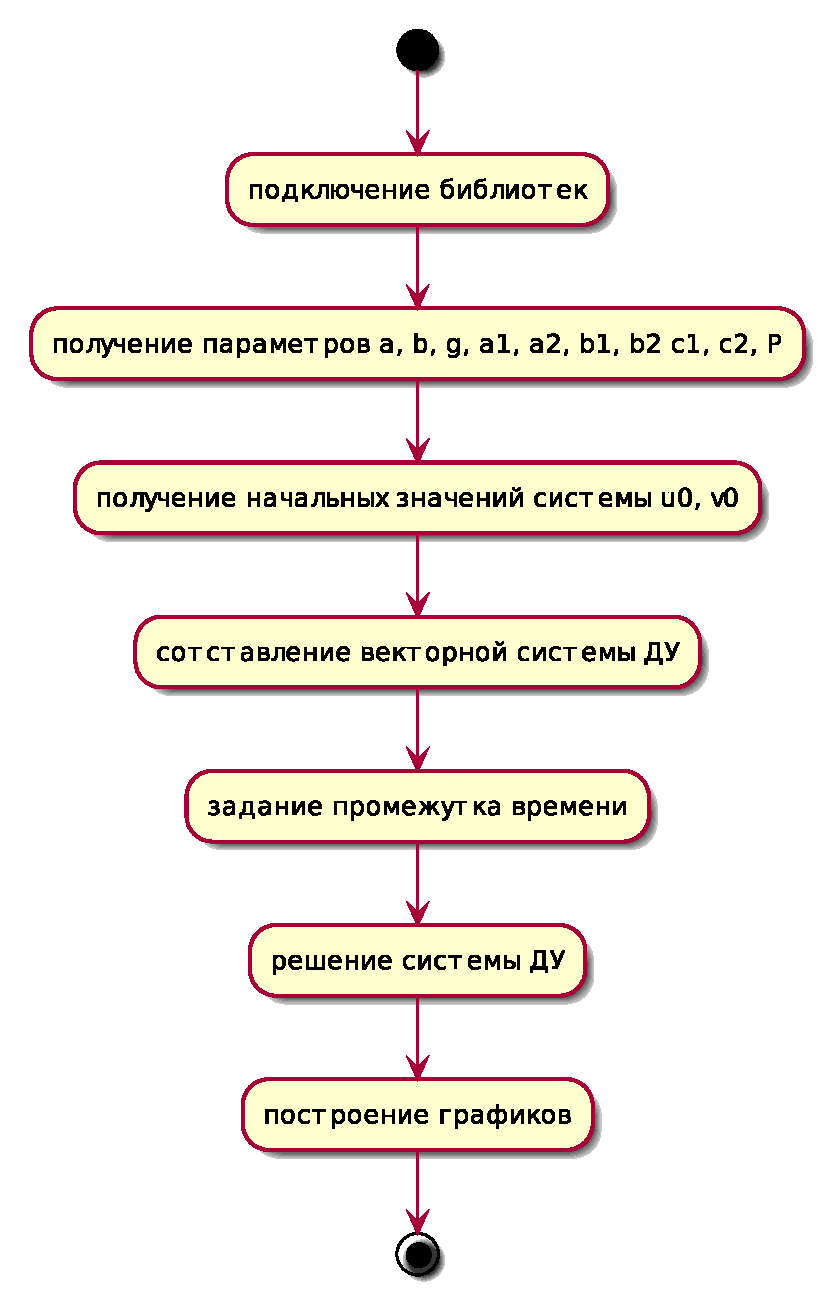
\includegraphics[width=0.65\textwidth,height=\textheight]{plantuml-images/b03e25730a3eeac3fcc1f4c9509882693fe1d580.eps}
\caption{Схема программы}\label{fig:main-program-diagram}
}
\end{figure}

\hypertarget{ux43fux43eux434ux433ux43eux442ux43eux432ux43aux430-ux442ux435ux441ux442ux43eux432ux44bux445-ux434ux430ux43dux43dux44bux445}{%
\section{Подготовка тестовых
данных}\label{ux43fux43eux434ux433ux43eux442ux43eux432ux43aux430-ux442ux435ux441ux442ux43eux432ux44bux445-ux434ux430ux43dux43dux44bux445}}

Модель описывается системой ДУ:

\[
\begin{cases}
\ \frac{du}{d\tau}=u(\frac{1+0.51*0}{1+1.2*0}-u\frac{1+0.51*0}{1+1.2*0})-\frac{uv}{1+2*u},\\
\ \frac{dv}{d\tau}=1*(-v\frac{1+0.510}{1+1.2*0}+5* \frac{uv}{1+2*u}).
\end{cases}
\]

Начальные условия: \(u_{0}=1, v_{0}=1\).

При \(P=0\), получается модель аналогичная исходной системе.

\[
\begin{cases}
\ \frac{du}{d\tau}=u(\frac{1+0.51*5}{1+1.2*5}-u\frac{1+0.51*5}{1+1.2*5})-\frac{uv}{1+2*u},\\
\ \frac{dv}{d\tau}=1*(-v\frac{1+0.51*5}{1+1.2*5}+5* \frac{uv}{1+2*u}).
\end{cases}
\]

Начальные условия: \(u_{0}=1, v_{0}=1\).

При \(P=5\), получается новая модель.

\hypertarget{ux43fux440ux430ux43aux442ux438ux447ux435ux441ux43aux430ux44f-ux447ux430ux441ux442ux44c-ux43aux443ux440ux441ux43eux432ux43eux439-ux440ux430ux431ux43eux442ux44b}{%
\chapter{Практическая часть курсовой
работы}\label{ux43fux440ux430ux43aux442ux438ux447ux435ux441ux43aux430ux44f-ux447ux430ux441ux442ux44c-ux43aux443ux440ux441ux43eux432ux43eux439-ux440ux430ux431ux43eux442ux44b}}

Результаты моделирования, проведённого в работе, четыре графика.

Первый и второй графики относятся к случаю \(P=0\) - Изменение
численности хищников и жертв при антропогенном давлении и фазовый
портрет.

Третий и четвертый графики относятся к случаю \(P=5\) - Изменение
численности хищников и жертв при антропогенном давлении и фазовый
портрет. Графические результаты (рис.
\ref{fig:1},\ref{fig:2},\ref{fig:3},\ref{fig:4}).

\begin{figure}
\hypertarget{fig:1}{%
\centering
\includegraphics[width=0.7\textwidth,height=\textheight]{1.png}
\caption{Изменение численности хищников и жертв при антропогенном
давлении в случае \(P=0\)}\label{fig:1}
}
\end{figure}

\begin{figure}
\hypertarget{fig:2}{%
\centering
\includegraphics[width=0.7\textwidth,height=\textheight]{2.png}
\caption{Фазовый портрет в случае \(P=0\)}\label{fig:2}
}
\end{figure}

\begin{figure}
\hypertarget{fig:3}{%
\centering
\includegraphics[width=0.7\textwidth,height=\textheight]{3.png}
\caption{Изменение численности хищников и жертв при антропогенном
давлении в случае \(P=5\)}\label{fig:3}
}
\end{figure}

\begin{figure}
\hypertarget{fig:4}{%
\centering
\includegraphics[width=0.7\textwidth,height=\textheight]{4.png}
\caption{Фазовый портрет в случае \(P=5\)}\label{fig:4}
}
\end{figure}

\hypertarget{ux437ux430ux43aux43bux44eux447ux435ux43dux438ux435}{%
\chapter*{Заключение}\label{ux437ux430ux43aux43bux44eux447ux435ux43dux438ux435}}
\addcontentsline{toc}{chapter}{Заключение}

В работе рассматривалась система дифференциальных уравнений, описывающих
взаимодействие двух популяций на загрязненной территории. Проводился
анализ системы на устойчивость методом Ляпунова.Построено четыре
графика, два из которых фазовые портреты.

\printbibliography[heading=bibintoc]

\appendix

\hypertarget{ux43aux43eux434-ux43fux440ux43eux433ux440ux430ux43cux43cux44b}{%
\chapter{Код
программы}\label{ux43aux43eux434-ux43fux440ux43eux433ux440ux430ux43cux43cux44b}}

\begin{minted}[xleftmargin=1em,linenos,autogobble]{julia}
using Pkg
using Plots
using DifferentialEquations
using ParameterizedFunctions
a = 2
b = 5
g = 1
a1 = 0.51
a2 = 1.2
b1 = 0.51
b2 = 1.2
c1 = 1.2
c2 = 0.51
P = 0
u0 = 1
v0 = 1
pp! = @ode_def PP begin
    du = u*((1+a1*P)/(1+a2*P) - u*(1+b2*P)/(1+b1*P)) - u*v/(1+a*u)
    dv = g*(-v*(1+c1*P)/(1+c2*P) + b*u*v/(1+a*u))
end a1 a2 b1 b2 c1 c2 
u = [u0,v0]
param=[a1, a2, b1, b2, c1, c2, a, b, g, P]
timespan = (0.0,100.0)
problem = ODEProblem(pp!, u, timespan, param)
solution = solve(problem)
plot(solution, title = "Predator - Prey model", xlabel = "t", ylabel = "u, v", label=["Prey (u)" "Predator (v)"])

plot(solution, vars=(1,2), xaxis="Prey", yaxis="Predator",legend=false)
\end{minted}

\end{document}
